%%Template made by Uday Khankhoje for examinations using the exam template
%%Refer to the documentation http://www-math.mit.edu/~psh/exam/examdoc.pdf 
%%for lot more bells and whistles to the standard template shown below
\documentclass[a4paper,11pt,addpoints]{exam}
\usepackage[left=1.5cm,right=1.5cm,top=1.5cm,bottom=2cm]{geometry}
%\usepackage{mathrsfs}
\usepackage{graphicx,color}
\usepackage[x11names]{xcolor}
\usepackage{venndiagram}
\usepackage{epic,eepic}
%\usepackage{mathpazo}
\usepackage{url}
\usepackage{tasks} % cria lista curta
\usepackage{multicol}
\usepackage{amsmath, amsthm, amssymb}
\pointsinmargin
\boxedpoints 
\renewcommand*\half{.5}
\usepackage{setspace}
\DeclareMathOperator{\vecc}{vec}
%\renewcommand{\vec}[1]{\ensuremath{\mathbf{#1}}}

\global\vbadness=1616

\begin{document}
\noindent 
%%PART 1 of header
\begin{center}
	\vspace*{-3em}
\def\arraystretch{2.0}
\begin{tabular}{|p{0.7\linewidth}|p{0.2\linewidth}|}
\hline 
\textbf{Avaliação de Matemática - Primeiro Bimestre} & Pontos Obtidos $\downarrow$ \\
\hline 
Data: 11.04.2023,\hspace{1cm}  Total de questões \textbf{\numquestions} \hspace{1cm} Total de pontos: \textbf{\numpoints} &   \\ 
\hline 
\multicolumn{2}{|l|}{Tuma: \hspace{0.3\linewidth} Nome: \hspace{0.3\linewidth} Duração: 2 hrs} \\
\hline
\end{tabular} 
\end{center}
%%PART 2 of header, if you have too many questions, this may be a problem
%%if so, use \multirowgradetable{n}[questions], where n is the number of rows you want
%%or, switch to \gradetable[h][pages] instead, 
\begin{center}
\gradetable[h][questions]
\end{center}
%%PART 3 of header
\textbf{Instruções
\begin{enumerate}
    \item Explique todas as questões claramente.
    \item Necessário todos os cálculos.
\end{enumerate}
}
%%toggle comment on next line to show/hide the answers
\printanswers
%%Now the actual paper!
\begin{questions}
\question[2] 
  Dados os conjuntos $A = \big\{-4,-3,-2,-1,0,1,2,3\big\}$, $B = \big\{-4,1,2,5,7\big\}$, $C = \big\{-1,0,1,2,3,4\big\}$ e $D = \big\{-2,-1,0,3,4,5,6,8\big\}$, determine:
  \begin{tasks}(2)
    \task $A \cup B$
    \task $A \cap B$
    \task $A - D$
    \task $(A \cup D) \cap (B - C)$
    \task $(A \cap D) - (B \cup C)$
  \end{tasks}

\begin{solution}[1in]
  \begin{tasks}
    \task $A \cup B = \big\{-4,-3,-2,-1,0,1,2,3,5,7\big\}$
    \task $A \cap B = \big\{-4,1,2\big\}$
    \task $A - D = \big\{-4,-3,1,2\big\}$
    \task $(A \cup D) \cap (B - C) = \big\{-4,-3,-2,-1,0,1,2,3,4,5,6,8\big\} \cap \big\{-4,5,7\big\} = \big\{-4,5\big\}$
    \task $(A \cap D) - (B \cup C) = \big\{-2,-1,0,3\big\} - \big\{-4,-1,0,1,2,3,4,5,7\big\} = \big\{-2\big\}$
  \end{tasks}
\end{solution}

\question[1]
  Sabendo que $A \cup B = \big\{1,2,4,6,8,10,12,14,16\big\}$, $A - B = \big\{1,2,10\big\}$ e $A \cap B = \big\{6, 8, 16\big\}$, represente os conjuntos \textit{A} e \textit{B} em um diagrama como este:

  \begin{center}
    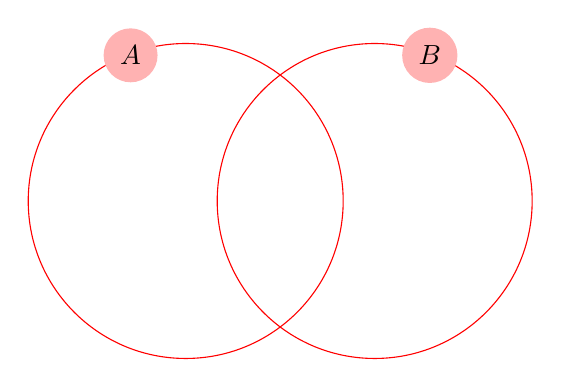
\begin{tikzpicture}

      \draw[red, thin] (0,0) circle[radius=2] node[black,circle,fill=red!30] at (-0.7,1.85) {$A$};
      \draw[red, thin] (2.4,0) circle[radius=2] node[black,circle,fill=red!30] at (3.1,1.85) {$B$};
      
    \end{tikzpicture}
  \end{center}

\begin{solution}
  \begin{center}
    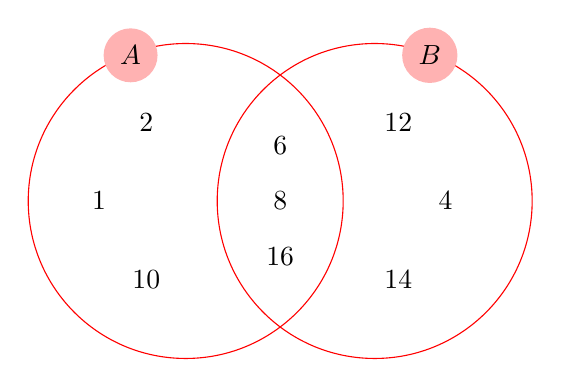
\begin{tikzpicture}

      \draw[red, thin] (0,0) circle[radius=2] node[black,circle,fill=red!30] at (-0.7,1.85) {$A$};
      \draw[red, thin] (2.4,0) circle[radius=2] node[black,circle,fill=red!30] at (3.1,1.85) {$B$};

      \node[black,thin] at (-1.1,0) {$1$};
      \node[black,thin] at (-0.5,1) {$2$};
      \node[black,thin] at (-0.5,-1) {$10$};

      \node[black,thin] at (1.2,0.7) {$6$};
      \node[black,thin] at (1.2,0) {$8$};
      \node[black,thin] at (1.2,-0.7) {$16$};
      
      \node[black,thin] at (3.3,0) {$4$};
      \node[black,thin] at (2.7,1) {$12$};
      \node[black,thin] at (2.7,-1) {$14$};

    \end{tikzpicture}
  \end{center}
\end{solution}

\question[1]

Represente, na reta real, os intervalos:

\begin{tasks}
  \task $A = \big[2, 8\big]$
  \task $B = \big\{x \in \mathbb{R} \,/\, 2 < x < 5\big\}$
  \task $C = \big]- \infty, 2\big]$
  \task $D = \big\{x \in \mathbb{R} \,/\, -2 \leq x \leq 2\big\}$
\end{tasks}

\begin{solution}[1in]

  \begin{tasks}
    \task {
      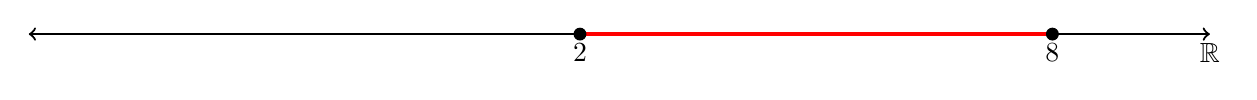
\begin{tikzpicture}
        \tikzstyle{aberto}=[fill=white, draw=black, circle, inner sep=1.5pt]
        \tikzstyle{fechado}=[fill=black, draw=black, circle, inner sep=1.5pt]

        \coordinate (A) at (-5,0);
        \coordinate (B) at (10,0);
        \coordinate (C) at (2,0);
        \coordinate (D) at (8,0);

        \draw[thick, <->] (A) -- (B);
        \draw[red, ultra thick] (C) -- (D);

        \node at (B)[below]{$\mathbb{R}$};

        \node at (C)[fechado]{};
        \node at (C)[below]{$2$};

        \node at (D)[fechado]{};
        \node at (D)[below]{$8$};
      \end{tikzpicture}
    }
    \task {
      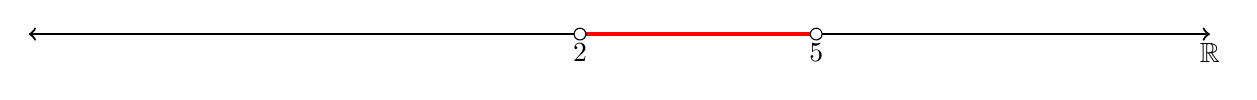
\begin{tikzpicture}
        \tikzstyle{aberto}=[fill=white, draw=black, circle, inner sep=1.5pt]
        \tikzstyle{fechado}=[fill=black, draw=black, circle, inner sep=1.5pt]

        \coordinate (A) at (-5,0);
        \coordinate (B) at (10,0);
        \coordinate (C) at (2,0);
        \coordinate (D) at (5,0);

        \draw[thick, <->] (A) -- (B);
        \draw[red, ultra thick] (C) -- (D);

        \node at (B)[below]{$\mathbb{R}$};

        \node at (C)[aberto]{};
        \node at (C)[below]{$2$};

        \node at (D)[aberto]{};
        \node at (D)[below]{$5$};
      \end{tikzpicture}
    }
    \task {
      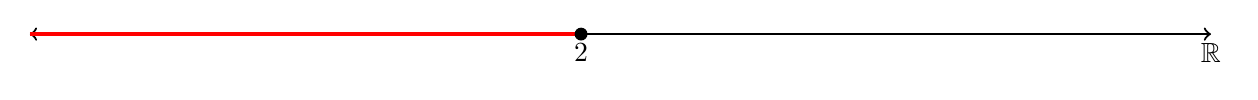
\begin{tikzpicture}
        \tikzstyle{aberto}=[fill=white, draw=black, circle, inner sep=1.5pt]
        \tikzstyle{fechado}=[fill=black, draw=black, circle, inner sep=1.5pt]

        \coordinate (A) at (-5,0);
        \coordinate (B) at (10,0);
        \coordinate (C) at (2,0);

        \draw[thick, <->] (A) -- (B);
        \draw[red, ultra thick] (A) -- (C);

        \node at (B)[below]{$\mathbb{R}$};

        \node at (C)[fechado]{};
        \node at (C)[below]{$2$};

      \end{tikzpicture}
    }
    \task {
      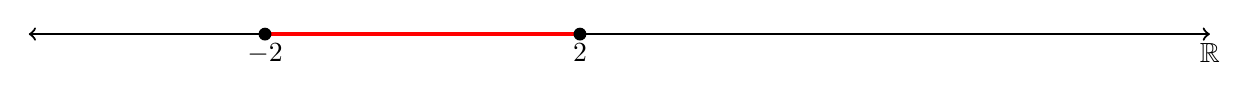
\begin{tikzpicture}
        \tikzstyle{aberto}=[fill=white, draw=black, circle, inner sep=1.5pt]
        \tikzstyle{fechado}=[fill=black, draw=black, circle, inner sep=1.5pt]

        \coordinate (A) at (-5,0);
        \coordinate (B) at (10,0);
        \coordinate (C) at (-2,0);
        \coordinate (D) at (2,0);

        \draw[thick, <->] (A) -- (B);
        \draw[red, ultra thick] (C) -- (D);

        \node at (B)[below]{$\mathbb{R}$};


        \node at (C)[fechado]{};
        \node at (C)[below]{$-2$};

        \node at (D)[fechado]{};
        \node at (D)[below]{$2$};
      \end{tikzpicture}
    }
  \end{tasks}

\end{solution}

\question[1]

Uma editora estuda a possibilidade de lançar novamente as publicações: \textit{Helena}, \textit{Senhora} e \textit{A Moreninha}. 
Para isto, efetuou uma pesquisa de mercado e concluiu que em cada 1000 pessoas consultas:

\begin{itemize}
  \item 600 leram \textit{A Moreninha};
  \item 400 leram \textit{Helena};
  \item 300 leram \textit{Senhora};
  \item 200 leram \textit{A Moreninha} e \textit{Helena};
  \item 150 leram \textit{A Moreninha} e \textit{Senhora};
  \item 100 leram \textit{Senhora} e \textit{Helena};
  \item 20 leram as três obras.
\end{itemize}

Calcule:

\begin{tasks}
  \task O número de pessoas que leu apenas uma das obras.
  \task O número de pessoas que não leu nenhuma das obras.
  \task O número de pessoas que leu duas ou mais obras.
\end{tasks}

\begin{solution}[1in]
  \begin{center}
    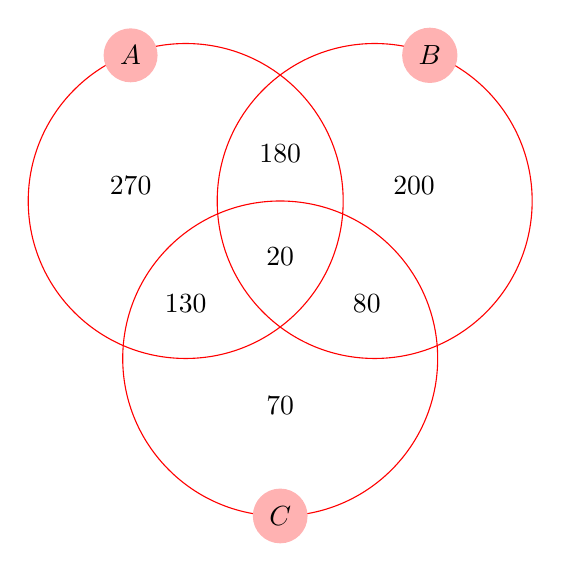
\begin{tikzpicture}

      \draw[red, thin] (0,0) circle[radius=2] node[black,circle,fill=red!30] at (-0.7,1.85) {$A$};
      \draw[red, thin] (2.4,0) circle[radius=2] node[black,circle,fill=red!30] at (3.1,1.85) {$B$};
      \draw[red, thin] (1.2,-2) circle[radius=2] node[black,circle,fill=red!30] at (1.2,-4) {$C$};

      \node[black,thin] at (-0.7,0.2) {$270$};
      \node[black,thin] at (1.2,0.6) {$180$};
      \node[black,thin] at (1.2,-0.7) {$20$};
      \node[black,thin] at (0,-1.3) {$130$};
      \node[black,thin] at (2.3,-1.3) {$80$};
      \node[black,thin] at (2.9,0.2) {$200$};
      \node[black,thin] at (1.2,-2.6) {$70$};

    \end{tikzpicture}
  \end{center}
  
  \begin{tasks}
    \task $270 + 70 + 200 = \boxed{540}$
    \task $1000 - (270+180+130+20+200+80+70) = 1000 - 950 = \boxed{50}$
    \task $130 + 20 + 180 + 80 = \boxed{410}$
  \end{tasks}
  
\end{solution}

\question[1]

Um funcionário do departamento de Recursos Humanos de uma indústria automobilística, analisando o currículo de 63 candidatos
a postos de trabalho, concluiu que apenas 5 deles nunca haviam trabalhado em montagem ou pintura, 37 já haviam trabalhado em 
montagem e 18 já haviam trabalhado nos dois setores. Quantos desses candidatos haviam trabalhado apenas em pintura?

\begin{solution}[2in]
  \begin{center}
    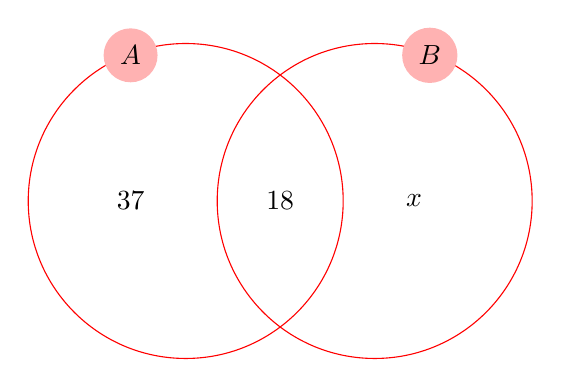
\begin{tikzpicture}

      \draw[red, thin] (0,0) circle[radius=2] node[black,circle,fill=red!30] at (-0.7,1.85) {$A$};
      \draw[red, thin] (2.4,0) circle[radius=2] node[black,circle,fill=red!30] at (3.1,1.85) {$B$};

      \node[black,thin] at (-0.7,0) {$37$};
      \node[black,thin] at (1.2,0) {$18$};
      \node[black,thin] at (2.9,0) {$x$};

    \end{tikzpicture}
  \end{center}

  $37 + 18 + x = 63 - 5 \implies \boxed{x = 3}$
\end{solution}

\question[1]

Em uma escola, numa turma de 40 estudantes, 26 jogam futebol, 15 jogam voleibol e 5 não praticam esporte algum. 
O número de alunos dessa turma que joga somente futebol é:
\begin{tasks}(5)
  \task 8
  \task 16
  \task 10
  \task 20
  \task 12
\end{tasks}

\begin{solution}[2in]
  \begin{center}
    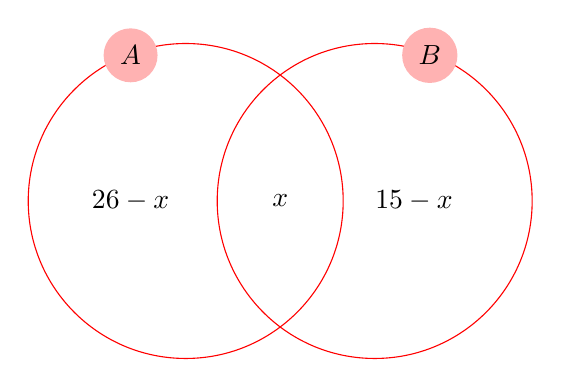
\begin{tikzpicture}

      \draw[red, thin] (0,0) circle[radius=2] node[black,circle,fill=red!30] at (-0.7,1.85) {$A$};
      \draw[red, thin] (2.4,0) circle[radius=2] node[black,circle,fill=red!30] at (3.1,1.85) {$B$};

      \node[black,thin] at (-0.7,0) {$26 - x$};
      \node[black,thin] at (1.2,0) {$x$};
      \node[black,thin] at (2.9,0) {$15 - x$};

    \end{tikzpicture}
  \end{center}


  $(26 - x) + x + (15 - x) = 40 - 5 \implies x = 6$

  $n(F - V) = n(F) - n(F \cap V) = 26 - 6 = \boxed{20}$
\end{solution}

\end{questions}
\end{document}
